% ==========================================================
%  Reinforcement Learning — Master Summary
%  Based on Sutton & Barto (2nd ed.) and lecture notes.
%  Template: see template.tex in repo root.
% ==========================================================

\documentclass[11pt, oneside]{book}


% ══════════════════════════════════════════════════════════
%  PAGE GEOMETRY
% ══════════════════════════════════════════════════════════
\usepackage[
  a4paper,
  top    = 2.6cm,
  bottom = 2.1cm,
  left   = 2.5cm,
  right  = 2.5cm,
  headheight = 15pt
]{geometry}


% ══════════════════════════════════════════════════════════
%  TYPOGRAPHY
% ══════════════════════════════════════════════════════════
\usepackage[T1]{fontenc}
\usepackage[utf8]{inputenc}
\usepackage{lmodern}
\usepackage{microtype}
\usepackage{inconsolata}

\setlength{\parindent}{0pt}
\setlength{\parskip}{0.62em}


% ══════════════════════════════════════════════════════════
%  MATHEMATICS
% ══════════════════════════════════════════════════════════
\usepackage{amsmath, amssymb, amsthm, mathtools}
\usepackage{bm}
\usepackage{bbm}
\usepackage{mathrsfs}
\usepackage{nicefrac}
\usepackage{cancel}


% ══════════════════════════════════════════════════════════
%  FIGURES, TABLES, LISTS
% ══════════════════════════════════════════════════════════
\usepackage{graphicx}
\usepackage{booktabs}
\usepackage{array}
\usepackage{float}
\usepackage{enumitem}

\setlist[itemize]{topsep=3pt, itemsep=2pt, leftmargin=2.2em}
\setlist[enumerate]{topsep=3pt, itemsep=2pt, leftmargin=2.4em}


% ══════════════════════════════════════════════════════════
%  COLORS
% ══════════════════════════════════════════════════════════
\usepackage{xcolor}

\definecolor{accent}{HTML}{1B3A5C}

\definecolor{def@frame}{HTML}{1A5276}   \definecolor{def@bg}{HTML}{EBF5FB}
\definecolor{thm@frame}{HTML}{922B21}   \definecolor{thm@bg}{HTML}{FDEDEC}
\definecolor{ex@frame} {HTML}{1E8449}   \definecolor{ex@bg} {HTML}{EAFAF1}
\definecolor{int@frame}{HTML}{9A6A00}   \definecolor{int@bg}{HTML}{FEF9E7}
\definecolor{note@frame}{HTML}{5B2C6F}  \definecolor{note@bg}{HTML}{F5EEF8}


% ══════════════════════════════════════════════════════════
%  CODE LISTINGS
% ══════════════════════════════════════════════════════════
\usepackage{listings}
\lstset{
  basicstyle       = \ttfamily\small,
  breaklines       = true,
  numbers          = left,
  numberstyle      = \tiny\color{gray!70},
  frame            = tb,
  framerule        = 0.4pt,
  rulecolor        = \color{gray!35},
  tabsize          = 2,
  showstringspaces = false,
  keywordstyle     = \color{def@frame}\bfseries,
  commentstyle     = \color{gray!55!black}\itshape,
  stringstyle      = \color{ex@frame!90!black},
  backgroundcolor  = \color{gray!5},
  xleftmargin      = 2em,
  xrightmargin     = 0.4em,
  aboveskip        = 0.8em,
  belowskip        = 0.5em
}


% ══════════════════════════════════════════════════════════
%  CUSTOM BOXES  (tcolorbox)
% ══════════════════════════════════════════════════════════
\usepackage[most]{tcolorbox}

\tcbset{
  enhanced,
  breakable,
  arc             = 2.5mm,
  boxrule         = 0.5pt,
  left            = 4.5mm,
  right           = 4mm,
  top             = 2.5mm,
  bottom          = 2.5mm,
  fonttitle       = \bfseries\small,
  sharp corners   = west,
  parbox          = false
}

\newtcolorbox{defbox}[1][]{
  title  = {Definition},
  colback = def@bg, colframe = def@frame,
  borderline west = {3.5pt}{0pt}{def@frame},
  #1
}

\newtcolorbox{thmbox}[1][]{
  title  = {Theorem / Key Formula},
  colback = thm@bg, colframe = thm@frame,
  borderline west = {3.5pt}{0pt}{thm@frame},
  #1
}

\newtcolorbox{exbox}[1][]{
  title  = {Example},
  colback = ex@bg, colframe = ex@frame,
  borderline west = {3.5pt}{0pt}{ex@frame},
  #1
}

\newtcolorbox{intbox}[1][]{
  title  = {Intuition \& Mental Model},
  colback = int@bg, colframe = int@frame,
  borderline west = {3.5pt}{0pt}{int@frame},
  #1
}

\newtcolorbox{notebox}[1][]{
  title  = {Note},
  colback = note@bg, colframe = note@frame,
  borderline west = {3.5pt}{0pt}{note@frame},
  #1
}


% ══════════════════════════════════════════════════════════
%  TABLE OF CONTENTS  (tocloft)
% ══════════════════════════════════════════════════════════
\usepackage[titles]{tocloft}

\renewcommand{\cftchapfont}     {\bfseries\color{accent}}
\renewcommand{\cftchappagefont} {\bfseries\color{accent}}
\renewcommand{\cftchapleader}   {\bfseries\color{accent!40}\cftdotfill{\cftdotsep}}
\setlength{\cftbeforechapskip} {7pt}

\renewcommand{\cftsecfont}      {\small}
\renewcommand{\cftsecpagefont}  {\small}
\setlength{\cftsecindent}      {1.8em}
\setlength{\cftbeforesecskip}  {1.5pt}

\renewcommand{\cftsubsecfont}      {\small\color{gray!65!black}}
\renewcommand{\cftsubsecpagefont}  {\small\color{gray!65!black}}
\setlength{\cftsubsecindent}      {3.4em}
\setlength{\cftbeforesubsecskip}  {0.5pt}


% ══════════════════════════════════════════════════════════
%  CHAPTER & SECTION HEADINGS  (titlesec)
% ══════════════════════════════════════════════════════════
\usepackage{titlesec}

\titleformat{\chapter}[display]
  {\normalfont\bfseries\color{accent}\huge}
  {\hfill\fontsize{68}{68}\selectfont\color{accent!13}\thechapter}
  {-10pt}
  {}
  [{\vspace{4pt}%
    {\color{accent}\rule{\linewidth}{1.6pt}}\\[-2pt]%
    {\color{accent!35}\rule{\linewidth}{0.5pt}}}]
\titlespacing*{\chapter}{0pt}{-28pt}{22pt}

\titleformat{\section}
  {\normalfont\large\bfseries\color{accent}}
  {\thesection}
  {0.8em}
  {}
  [{\vspace{1pt}\color{accent!45}\titlerule[0.45pt]}]
\titlespacing*{\section}{0pt}{3.8ex plus 1ex minus .2ex}{2.2ex plus .2ex}

\titleformat{\subsection}
  {\normalfont\normalsize\bfseries\color{accent!80!black}}
  {\thesubsection}
  {0.7em}
  {}
\titlespacing*{\subsection}{0pt}{2.6ex plus 1ex minus .2ex}{1.4ex plus .2ex}

\titleformat{\paragraph}[runin]
  {\normalfont\small\bfseries}
  {}
  {0em}
  {}[.\enspace]
\titlespacing{\paragraph}{0pt}{1.2ex plus .5ex minus .2ex}{0.5em}


% ══════════════════════════════════════════════════════════
%  HEADER & FOOTER
% ══════════════════════════════════════════════════════════
\usepackage{fancyhdr}
\pagestyle{fancy}
\fancyhf{}
\fancyhead[L]{\small\color{gray!70}\nouppercase{\leftmark}}
\fancyhead[R]{\small\color{gray!70}\thepage}
\renewcommand{\headrulewidth}{0.4pt}

\fancypagestyle{plain}{%
  \fancyhf{}
  \fancyfoot[C]{\small\color{gray!70}\thepage}
  \renewcommand{\headrulewidth}{0pt}%
}


% ══════════════════════════════════════════════════════════
%  LINKS & REFERENCES
% ══════════════════════════════════════════════════════════
\usepackage[hidelinks]{hyperref}
\usepackage[nameinlink, capitalize]{cleveref}


% ══════════════════════════════════════════════════════════
%  DOCUMENT METADATA
% ══════════════════════════════════════════════════════════
\newcommand{\coursetitle}{Reinforcement Learning}
\newcommand{\documenttype}{Master Summary}
\newcommand{\authorname}{Stefan Eder}
\newcommand{\basedon}{Based on Sutton \& Barto (2nd ed.) and lecture notes}


% ══════════════════════════════════════════════════════════
%  MATHEMATICAL MACROS
% ══════════════════════════════════════════════════════════

% ── Number Sets & Spaces ──────────────────────────────────
\newcommand{\R}{\mathbb{R}}
\newcommand{\Nats}{\mathbb{N}}
\newcommand{\Z}{\mathbb{Z}}
\newcommand{\C}{\mathbb{C}}

% ── Probability & Statistics ──────────────────────────────
\newcommand{\E}{\mathbb{E}}
\newcommand{\Prob}{\mathbb{P}}
\newcommand{\Var}{\mathrm{Var}}
\newcommand{\Cov}{\mathrm{Cov}}
\newcommand{\ind}{\mathbbm{1}}

% ── Calculus & Optimization ───────────────────────────────
\newcommand{\argmax}{\operatorname*{arg\,max}}
\newcommand{\argmin}{\operatorname*{arg\,min}}
\newcommand{\dd}{\,\mathrm{d}}
\newcommand{\pd}[2]{\frac{\partial #1}{\partial #2}}

% ── Norms & Inner Products ────────────────────────────────
\newcommand{\norm}[1]{\left\lVert #1 \right\rVert}
\newcommand{\abs}[1]{\left\lvert #1 \right\rvert}

% ── Linear Algebra ────────────────────────────────────────
\newcommand{\T}{^{\mathsf{T}}}

% ── ML / AI Core ─────────────────────────────────────────
\newcommand{\params}{\boldsymbol{\theta}}
\newcommand{\loss}{\mathcal{L}}
\DeclareMathOperator{\softmax}{softmax}

% ── Reinforcement Learning ────────────────────────────────
\newcommand{\Sset}{\mathcal{S}}          % State space
\newcommand{\Aset}{\mathcal{A}}          % Action space
\newcommand{\vpi}{v_{\pi}}              % State-value under policy \pi
\newcommand{\qpi}{q_{\pi}}             % Action-value under policy \pi
\newcommand{\vstar}{v_{*}}             % Optimal state-value function
\newcommand{\qstar}{q_{*}}            % Optimal action-value function
\newcommand{\qtrue}{q_{*}}            % True action value (bandit context)


% ==========================================================
%  BEGIN DOCUMENT
% ==========================================================
\begin{document}

\frontmatter


% ──────────────────────────────────────────────────────────
%  TITLE PAGE
% ──────────────────────────────────────────────────────────
\thispagestyle{empty}
\vspace*{1.8cm}

\begin{center}
  {\color{accent}\rule{\linewidth}{1.8pt}}
  \vspace{0.65cm}

  {\fontsize{28}{34}\selectfont\bfseries\color{accent}\coursetitle\par}
  \vspace{0.25cm}
  {\large\color{gray!80!black}\documenttype\par}

  \vspace{0.55cm}
  {\color{accent!35}\rule{\linewidth}{0.5pt}}
  \vspace{0.55cm}

  {\large\authorname\par}
  \vspace{0.2cm}
  {\small\color{gray!70}\basedon\par}
\end{center}

\vspace{1.6cm}

\begin{center}
\begin{minipage}{0.84\textwidth}
  \small\color{gray!80!black}
  This document is a compact summary of the Reinforcement Learning course,
  covering finite MDPs, bandits, dynamic programming, Monte Carlo methods,
  temporal-difference learning, and policy gradient methods.
  It is designed as a study aid alongside the textbook and lecture notes,
  not as a replacement for them.

  \medskip
  If you spot an error or a gap, please open an issue or pull request at
  \textbf{github.com/stevetgit} --- corrections are always welcome.

  \medskip
  \color{gray!60!black}
  Good study materials should be shared, not gatekept.
  If this helped you, take it as a reason to help the next colleague you see struggling.
\end{minipage}
\end{center}

\vfill
{\centering\small\color{gray!65} \today\par}
\clearpage


% ──────────────────────────────────────────────────────────
%  TABLE OF CONTENTS
% ──────────────────────────────────────────────────────────
\setcounter{tocdepth}{2}

\begingroup
  \let\cleardoublepage\relax
  \let\clearpage\relax
  \tableofcontents
\endgroup

\mainmatter


% ==========================================================
\chapter{Finite Markov Decision Processes}
% ==========================================================

Reinforcement learning (RL) is the third major learning paradigm alongside
supervised and unsupervised learning. In \textbf{supervised learning} we fit a
mapping $x\mapsto y$ from labeled pairs; in \textbf{unsupervised learning} we
discover structure in unlabeled data. RL is different: an \textbf{agent}
interacts with an \textbf{environment} and learns to act so as to maximize
cumulative reward. The environment is not a fixed dataset --- it responds to
the agent's actions, which makes the exploration--exploitation trade-off
central to RL in a way that simply does not arise in the other two paradigms.

\section{The agent--environment interface}

At each discrete time step $t = 0, 1, 2, \dots$ the agent observes the
current state, chooses an action, and the environment returns a reward and a
new state.

\begin{defbox}[title={Trajectory}]
The agent observes state $S_t \in \Sset$ and selects action $A_t \in \Aset(S_t)$.
The environment responds with reward $R_{t+1} \in \R$ and next state $S_{t+1}$.
The resulting sequence
\[
  S_0,\; A_0,\; R_1,\; S_1,\; A_1,\; R_2,\; \dots
\]
is called a \emph{trajectory} (or history).
\end{defbox}

\begin{figure}[h]
  \centering
  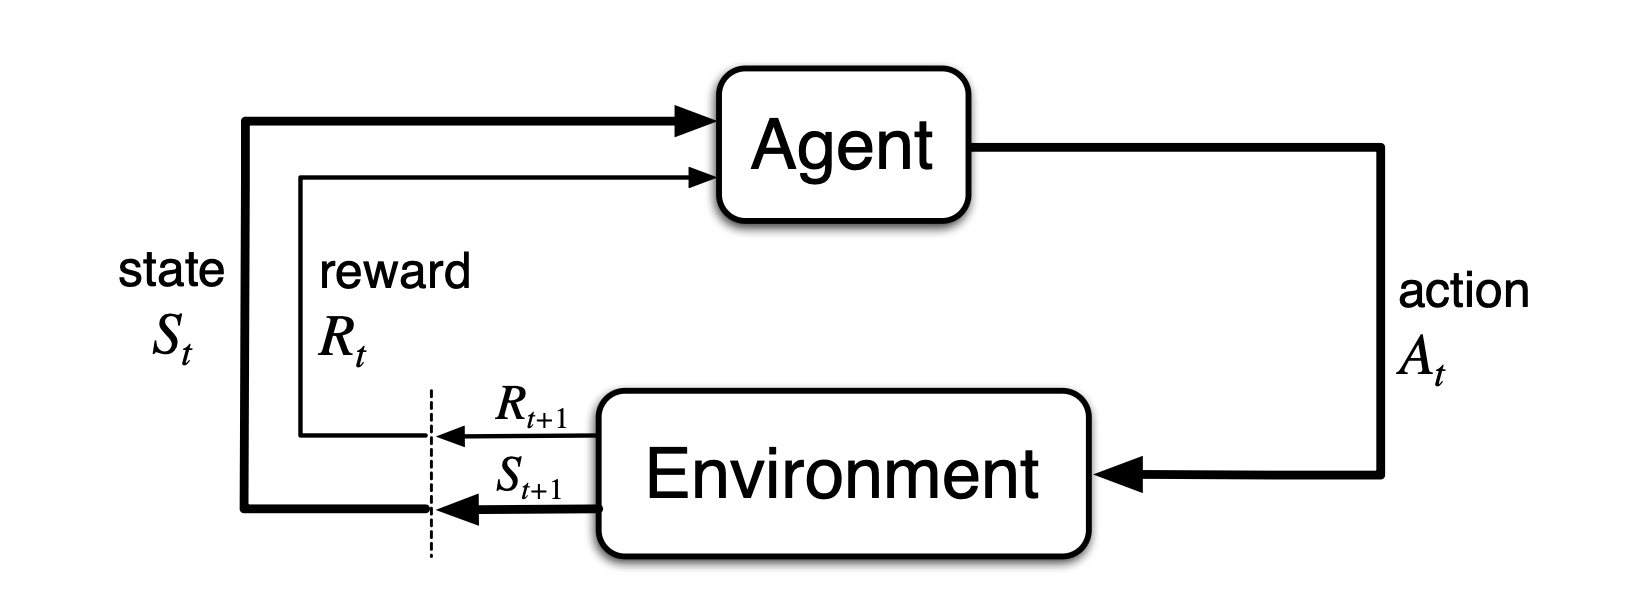
\includegraphics[width=0.85\linewidth]{figures/agent-environment.png}
  \caption{Standard agent--environment interaction at time $t$.}
  \label{fig:agent-env}
\end{figure}

The agent's behavior is encoded in a \emph{policy}.

\begin{defbox}[title={Policy}]
A \emph{policy} $\pi$ specifies how the agent acts.
In the most general (stochastic) case,
\[
  \pi(a \mid s) \;=\; \Pr(A_t = a \mid S_t = s).
\]
A policy is \emph{deterministic} if it selects a single action with
probability 1 in each state.
\end{defbox}

\section{Markov property and MDP dynamics}

The Markov property makes the state a sufficient statistic for future
behavior: knowing the present state is enough; the history adds nothing.

\begin{defbox}[title={Markov Property}]
A state signal is \emph{Markov} if the next-state and reward distribution
depends on the past only through the current state and action:
\[
  \Pr(S_{t+1}=s', R_{t+1}=r \mid S_t=s, A_t=a,\;\text{past})
  \;=\;
  \Pr(S_{t+1}=s', R_{t+1}=r \mid S_t=s, A_t=a).
\]
\end{defbox}

A classic illustration: if the state is the full chess board position, the
next position depends only on that board and the move --- Markov.
If instead the state were only the knight's current square (ignoring the rest
of the board), it would \emph{not} be Markov, because the hidden pieces still
influence what moves are legal.

A state space can be discrete (countably many states, e.g.\ chess positions)
or continuous (uncountably many, e.g.\ real-valued sensor readings).
The complete model of how the environment transitions is given by the
\emph{dynamics function}.

\begin{defbox}[title={Finite MDP}]
A \textbf{finite Markov decision process (finite MDP)} is defined by finite
state and action sets together with the \emph{dynamics}
\[
  p(s', r \mid s, a) \;=\; \Pr(S_{t+1}=s',\, R_{t+1}=r \mid S_t=s,\, A_t=a).
\]
Derived quantities used throughout:
\[
  r(s,a) = \E[R_{t+1}\mid S_t=s, A_t=a],
  \qquad
  p(s'\mid s,a) = \Pr(S_{t+1}=s'\mid S_t=s, A_t=a).
\]
Intuitively, $p$ is the environment's rulebook: ``if you do $a$ in $s$, what
tends to happen next?''
\end{defbox}

\begin{figure}[h]
  \centering
  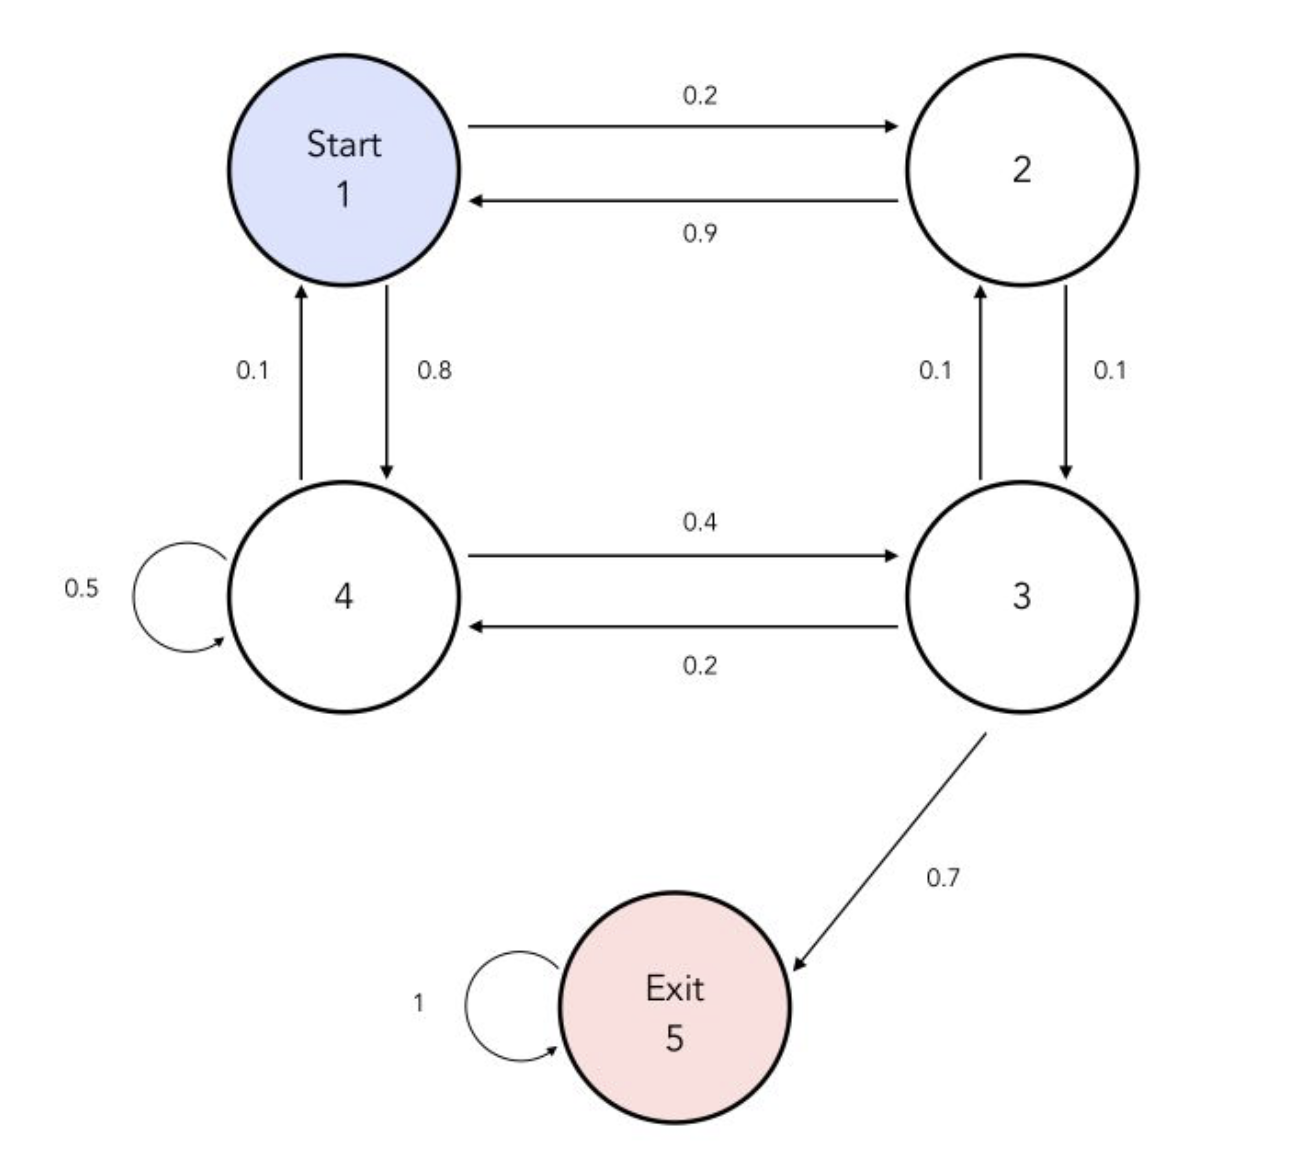
\includegraphics[scale=0.4]{figures/transition.png}
  \caption{A small MDP visualized as a directed graph with action-labeled transitions.}
  \label{fig:mdp-graph}
\end{figure}

\section{Goals, rewards, and returns}

The \textbf{reward hypothesis} states that all goals can be formalized as
maximizing a cumulative scalar reward signal. The reward $R_{t+1}$ is the
immediate feedback; what the agent actually cares about is the long-run sum.
Importantly, reward is a \emph{design choice}, not synonymous with
``winning'': for chess one might use $+1$ win, $0$ draw, $-1$ loss; for
navigation, $-1$ per time step and $0$ at the goal encourages the shortest
path; for robotics, shaping the reward incorrectly can lead to unintended
behavior.

\begin{defbox}[title={Return and Discount Factor}]
For an \textbf{episodic task} that terminates at time $T$, the
\textbf{discounted return} from time $t$ is
\[
  G_t \;=\; \sum_{k=0}^{T-t-1} \gamma^k R_{t+k+1},
\]
where $\gamma \in [0,1]$ is the \textbf{discount factor}.
For a \textbf{continuing task} (no terminal time), discounting with
$\gamma < 1$ keeps the infinite sum finite and expresses preference for
sooner rewards.
\end{defbox}

A key identity simplifies computing returns backward through an episode:
\[
  G_t = R_{t+1} + \gamma G_{t+1}.
\]
Starting from $G_T = 0$ and iterating back is far more efficient than summing
forward from each $t$. As a sanity check: for a continuing task with constant
reward $R_{t+1} = r$ and $\gamma \in [0,1)$, the geometric series gives
$G_t = r/(1-\gamma)$.

\section{Value functions}

Value functions answer the question: ``how good is it to be in state $s$ (or
to take action $a$ in $s$) under a given policy?'' They are the central
objects computed and approximated throughout RL.

\begin{defbox}[title={State-Value and Action-Value Functions}]
Given a policy $\pi$, the \textbf{state-value function} and
\textbf{action-value function} are
\[
  \vpi(s) = \E_{\pi}[G_t \mid S_t=s],
  \qquad
  \qpi(s,a) = \E_{\pi}[G_t \mid S_t=s, A_t=a].
\]
Intuitively: $\vpi(s)$ is how good it is to be in $s$ under $\pi$;
$\qpi(s,a)$ is how good it is to take $a$ in $s$ and then follow $\pi$.
\end{defbox}

Both value functions satisfy recursive \emph{Bellman equations} that express
current value as one-step reward plus discounted future value.

\begin{thmbox}[title={Bellman Expectation Equations}]
For a finite MDP under policy $\pi$:
\[
  \vpi(s)
  = \sum_{a}\pi(a\mid s)\sum_{s',r} p(s',r\mid s,a)\bigl[r + \gamma\,\vpi(s')\bigr],
\]
\[
  \qpi(s,a)
  = \sum_{s',r} p(s',r\mid s,a)
    \Bigl[r + \gamma\underbrace{\sum_{a'}\pi(a'\mid s')\,\qpi(s',a')}_{=\;\vpi(s')}\Bigr].
\]
Reading the first equation: ``value equals expected immediate reward plus
discounted value of the next state.''
\end{thmbox}

\section{Optimal value functions and Bellman optimality}

A policy $\pi$ is \emph{optimal} if $\vpi(s) \ge v_{\pi'}(s)$ for all $s$
and all policies $\pi'$. Such a policy always exists for finite MDPs.

\begin{defbox}[title={Optimal Value Functions}]
\[
  \vstar(s) = \max_{\pi} \vpi(s),
  \qquad
  \qstar(s,a) = \max_{\pi} \qpi(s,a).
\]
An optimal policy $\pi_*$ attains these maxima simultaneously for all $s$.
\end{defbox}

The optimal value functions are the unique solutions to the Bellman
\emph{optimality} equations, which replace the policy-weighted sum by a
\emph{max}:

\begin{thmbox}[title={Bellman Optimality Equations}]
\[
  \vstar(s) = \max_{a}\sum_{s',r} p(s',r\mid s,a)\bigl[r + \gamma\,\vstar(s')\bigr],
\]
\[
  \qstar(s,a) = \sum_{s',r} p(s',r\mid s,a)\bigl[r + \gamma\max_{a'}\qstar(s',a')\bigr].
\]
A greedy policy w.r.t.\ $\qstar$ is optimal:
$\pi_*(s) \in \argmax_a\,\qstar(s,a)$.
\end{thmbox}

\section{Exam questions}

\begin{exbox}[title={Exam: Matching Concepts}]
\textbf{Q.} Match each description to the correct concept:
(A) defines the agent's behavior at a given time,
(B) mimics the behavior of the environment,
(C) immediate scalar feedback provided each step,
(D) expected sum of future rewards indicating long-term desirability.
Concepts: (1) policy, (2) model, (3) reward signal, (4) value function.

\medskip
\textbf{A.} A $\to$ policy,\quad B $\to$ model,\quad C $\to$ reward signal,\quad D $\to$ value function.
\end{exbox}

\begin{exbox}[title={Exam: Return Computation}]
\textbf{Q.} Let $\gamma = \tfrac{1}{2}$ and rewards $R_1=-7,\,R_2=6,\,R_3=1,\,R_4=5,\,R_5=2$
with terminal time $T=5$. Compute $G_0,\dots,G_5$.

\medskip
\textbf{A.} Work backward using $G_t = R_{t+1} + \gamma G_{t+1}$ and $G_5=0$:
\[
  G_4=2,\quad G_3=5+\tfrac12\cdot2=6,\quad G_2=1+\tfrac12\cdot6=4,
\]
\[
  G_1=6+\tfrac12\cdot4=8,\quad G_0=-7+\tfrac12\cdot8=-3.
\]
\end{exbox}

\begin{exbox}[title={Exam: Undiscounted Return for Non-Episodic Tasks}]
\textbf{Q.} ``It is better to use the undiscounted return ($\gamma=1$) for
non-episodic tasks.'' True or false?

\medskip
\textbf{A.} \textbf{False in general.} For continuing tasks, an undiscounted
infinite sum can diverge. Typical fixes: $\gamma < 1$ (bounded rewards), or
an average-reward objective.
\end{exbox}


% ==========================================================
\chapter{Multi-Armed Bandits}
% ==========================================================

The multi-armed bandit is the simplest setting where the
exploration--exploitation trade-off appears in pure form. There is no state
transition: the agent simply picks an arm at each step and observes a reward.
Despite this simplicity, bandits introduce every key idea needed for the
full RL setting.

\section{Problem setup}

\begin{defbox}[title={$k$-Armed Bandit}]
A \textbf{$k$-armed bandit} has $k$ actions (arms) $a \in \{1,\dots,k\}$.
At each time step $t$ the agent selects $A_t$ and observes reward $R_t$.
The \textbf{true value} of arm $a$ (stationary case) is
\[
  \qtrue(a) \;=\; \E[R_t \mid A_t = a].
\]
The agent maintains an \textbf{estimate} $Q_t(a)$ and a \textbf{count}
$N_t(a)$ = number of times arm $a$ has been selected up to time $t$.
\end{defbox}

A problem is \textbf{stationary} if $\qtrue(a)$ is constant over time;
\textbf{non-stationary} if the reward distributions drift. This distinction
drives the choice of update rule later.

\section{Exploration vs.\ exploitation}

\textbf{Exploitation} selects the arm with the highest current estimate
(greedy w.r.t.\ $Q_t$), extracting maximum immediate reward given current
knowledge. \textbf{Exploration} instead tries other arms to improve estimates,
accepting lower short-term reward for potentially better long-term performance.
You cannot do both simultaneously; the trade-off is the central problem of bandits.

\section{Action-value methods}

The sample-average estimate is the natural unbiased estimator:

\begin{thmbox}[title={Sample-Average Estimate}]
If arm $a$ has been selected $N_t(a) \ge 1$ times:
\[
  Q_t(a) = \frac{1}{N_t(a)}\sum_{i=1}^{N_t(a)} R^{(i)}(a).
\]
\end{thmbox}

Computing this from scratch each step is wasteful. The incremental form
processes one new observation at a time:

\begin{thmbox}[title={Incremental Update (ISAM)}]
After selecting $A_t$ and observing $R_t$, update only $Q(A_t)$:
\[
  Q_{t+1}(A_t) = Q_t(A_t) + \frac{1}{N_{t+1}(A_t)}\bigl(R_t - Q_t(A_t)\bigr).
\]
More generally, with a constant step size $\alpha \in (0,1]$:
\[
  Q_{t+1}(A_t) = Q_t(A_t) + \alpha\bigl(R_t - Q_t(A_t)\bigr).
\]
The constant-$\alpha$ version is an \textbf{exponentially recency-weighted}
average --- ideal for non-stationary problems where older rewards should count
less.
\end{thmbox}

\begin{exbox}[title={Incremental Update Calculation}]
If $Q_t(a) = -3$, $R_t = 2$, $\alpha = 0.1$:
\[
  Q_{t+1}(a) = -3 + 0.1\bigl(2 - (-3)\bigr) = -3 + 0.5 = -2.5.
\]
\end{exbox}

\section{$\varepsilon$-greedy}

\begin{defbox}[title={$\varepsilon$-Greedy Action Selection}]
With probability $1 - \varepsilon$ choose the greedy action
$A_t \in \argmax_a Q_t(a)$, and with probability $\varepsilon$ choose
uniformly at random from $\{1,\dots,k\}$.
\end{defbox}

With constant $\varepsilon > 0$, exploration never stops: a fraction
$\varepsilon$ of steps will forever be random. Smaller $\varepsilon$ typically
yields higher asymptotic reward but slower early learning. Pure greedy
($\varepsilon=0$) can get stuck on a suboptimal arm because early noise drives
it to commit before all arms are tried. \textbf{GLIE} schedules (Greedy in
the Limit with Infinite Exploration, e.g.\ $\varepsilon_k = 1/k$) decay
$\varepsilon$ to zero while still exploring infinitely often --- a condition
required for convergence guarantees.

\begin{exbox}[title={Greedy Selection Probability}]
Under $\varepsilon$-greedy with uniform exploration, the probability of
selecting the greedy action is
\[
  \Pr(\text{greedy}) = (1-\varepsilon) + \frac{\varepsilon}{k}.
\]
For $k=10$, $\varepsilon = 0.7$: $\Pr(\text{greedy}) = 0.3 + 0.07 = 0.37$.

Note: if a \emph{non-greedy} action was selected, the $\varepsilon$-branch
definitely fired. If the greedy action was selected, it could have come from
either branch.
\end{exbox}

\section{Optimistic initial values}

\begin{intbox}[title={Optimistic Initialization}]
Set $Q_1(a)$ to values \emph{higher} than any plausible reward (requiring
rough knowledge of the reward scale). Under pure greedy selection, untried
arms keep their optimistic estimates and will therefore be selected, driving
early exploration without any randomness.

Works well in \textbf{stationary} environments. In non-stationary settings
the initial optimism is ``washed out'' once values converge: if rewards then
shift, the mechanism provides no further exploration.
\end{intbox}

\begin{notebox}[title={Exam Nuances: Exploration Hyperparameters}]
\begin{itemize}
  \item \textbf{$\varepsilon$-greedy} controls exploration explicitly via
    $\varepsilon$: larger $\varepsilon \Rightarrow$ more random steps.
  \item \textbf{UCB} controls exploration via $c$: larger $c \Rightarrow$
    larger uncertainty bonus.
  \item \textbf{Optimistic initialization} requires a reward-scale prior
    (an implicit, one-time exploration parameter), but does not expose a
    run-time knob.
  \item \textbf{Gradient bandits} have no explicit exploration rate. They
    explore because they \emph{sample} from a softmax. The step size
    $\alpha$ controls learning speed, not exploration probability.
\end{itemize}
If rewards are strictly negative, $Q_1(a) = 0$ is already optimistic.
\end{notebox}

\section{Upper Confidence Bound (UCB)}

\begin{thmbox}[title={UCB Action Selection}]
\[
  A_t \in \argmax_a \left[Q_t(a) + c\sqrt{\frac{\ln t}{N_t(a)}}\right],
\]
where $c > 0$ controls exploration. Each action is selected at least once
before the formula is applied, so $N_t(a) \ge 1$.
Setting $c = 0$ reduces UCB to pure greedy.
\end{thmbox}

Note that UCB naturally revisits neglected arms: if arm $a$ is skipped for
a while, $N_t(a)$ stays constant while $\ln t$ grows, so the bonus slowly
\emph{increases} until the arm becomes attractive again.

\begin{intbox}[title={Why the UCB Bonus Works}]
The bonus $c\sqrt{\ln t / N_t(a)}$ is large when arm $a$ is uncertain (small
$N_t(a)$), making UCB ``optimistic in the face of uncertainty.'' As $a$ is
sampled more, $N_t(a)$ grows and the bonus shrinks --- once you are confident
an arm is bad, it stops looking attractive.

UCB therefore explores \emph{selectively}, prioritizing arms where evidence
is weak and a surprise could still happen. In contrast, $\varepsilon$-greedy
explores uniformly at random regardless of confidence. The $\ln t$ numerator
slowly increases pressure to re-examine arms, but the growth is dominated by
$N_t(a)$, so focus naturally shifts from exploration to exploitation over
time.

In short: \textbf{explore what you are unsure about; exploit what you are
confident is good.}
\end{intbox}

The classic UCB derivation assumes \textbf{stationary} bandits. In strongly
non-stationary settings, modifications such as sliding-window or discounted
UCB are needed.

\section{Non-stationary problems}

When $\qtrue(a)$ drifts over time, the sample average gives equal weight to
all past observations --- including stale ones. The constant step-size rule
$Q_{t+1}(A_t) = Q_t(A_t) + \alpha(R_t - Q_t(A_t))$ with fixed $\alpha$
exponentially downweights older rewards, letting the estimate track changes.
This comes at the cost of never fully converging even in stationary settings.

\section{Gradient bandits}

\begin{defbox}[title={Preference Parameters}]
Instead of estimating action values, gradient bandits maintain a real-valued
\textbf{preference} (logit) $H_t(a) \in \R$ for each arm. Only
\emph{differences} matter: adding a constant to all $H_t(a)$ leaves the
policy unchanged. Large $H_t(a)$ means the policy is more likely to pick $a$.
\end{defbox}

Preferences are converted to action probabilities by the softmax:

\begin{thmbox}[title={Softmax Policy and Gradient Update}]
\[
  \pi_t(a) = \frac{\exp(H_t(a))}{\sum_b \exp(H_t(b))}.
\]
Actions are sampled from $\pi_t(\cdot)$ (not greedy). After observing
$R_t$ with baseline $\bar{R}_t$ (often the running average reward):
\[
  H_{t+1}(a) =
  \begin{cases}
    H_t(a) + \alpha(R_t - \bar{R}_t)(1 - \pi_t(a)) & a = A_t, \\[4pt]
    H_t(a) - \alpha(R_t - \bar{R}_t)\,\pi_t(a) & a \ne A_t.
  \end{cases}
\]
\end{thmbox}

\begin{intbox}[title={What the Gradient Update Is Doing}]
Think of $\pi_t$ as a weighted lottery. After picking $A_t$:
\begin{itemize}
  \item If $R_t > \bar{R}_t$ (better than average): increase $H(A_t)$, making
    $A_t$ more likely; decrease others slightly.
  \item If $R_t < \bar{R}_t$ (worse than average): decrease $H(A_t)$;
    increase others slightly.
\end{itemize}
The factors $(1 - \pi_t(A_t))$ and $\pi_t(a)$ scale the update: large
adjustments when the action was unlikely (surprising), small adjustments when
it was already highly probable. This is gradient ascent on expected reward
w.r.t.\ the preference parameters.
\end{intbox}

\begin{notebox}[title={Key Distinctions}]
\textbf{Preferences $\ne$ value estimates:} $H_t(a)$ defines $\pi_t$ via
softmax; it is \emph{not} an estimate of $Q(a)$.

\textbf{Baseline must be action-independent:} using $Q_t(A_t)$ as a baseline
is generally invalid. A valid action-independent baseline is
$\sum_a \pi_t(a) Q_t(a)$ (the expected value under the current policy).

\textbf{Exam wording trap:} ``actions are selected proportional to their
preference'' is technically false ($\pi_t(a) \propto \exp(H_t(a))$, not
$\propto H_t(a)$). Past exams have marked this \textbf{True}, treating
``preference'' loosely as the softmax sense.
\end{notebox}

\section{Exam questions}

\begin{exbox}[title={Exam: Optimistic Initialization}]
\textbf{Q.} ``Optimistic initial values bias the agent toward exploring
actions with higher estimated rewards.'' True or false?

\medskip
\textbf{A.} \textbf{True.} Untried arms keep optimistic estimates; greedy
selection is therefore drawn to them first.
\end{exbox}

\begin{exbox}[title={Exam: UCB}]
\textbf{Q.} ``UCB balances exploration and exploitation by adding an
uncertainty term to each action value.'' True or false?

\medskip
\textbf{A.} \textbf{True.} The defining idea is
$\argmax_a\bigl[Q_t(a) + \text{bonus}(a)\bigr]$.
\end{exbox}

\begin{exbox}[title={Exam: Gradient Bandits}]
\textbf{Q.} ``In gradient bandits, actions are selected proportional to their
action preference.'' True or false?

\medskip
\textbf{A.} \textbf{True} (as marked in past exams, using ``preference'' in
the softmax sense: $\pi_t(a) \propto \exp(H_t(a))$). Strictly, proportional
to the \emph{exponentiated} preference.
\end{exbox}


% ==========================================================
\chapter{Dynamic Programming}
% ==========================================================

Dynamic programming (DP) in RL refers to a family of \emph{planning}
algorithms: they compute value functions and optimal policies using a
\textbf{known MDP model} $p(s',r\mid s,a)$. Because the model is available,
DP performs \textbf{expected backups} (sums over all possible next states)
rather than learning from sampled experience. This makes DP exact but
inapplicable whenever the model is unknown.

Three terms appear throughout:
a \textbf{backup} updates one value $V(s)$ using the Bellman equation;
a \textbf{sweep} is one pass that performs at most one backup per state
$s \in \Sset$;
\textbf{iterative evaluation} repeats sweeps until convergence.

\begin{figure}[h]
  \centering
  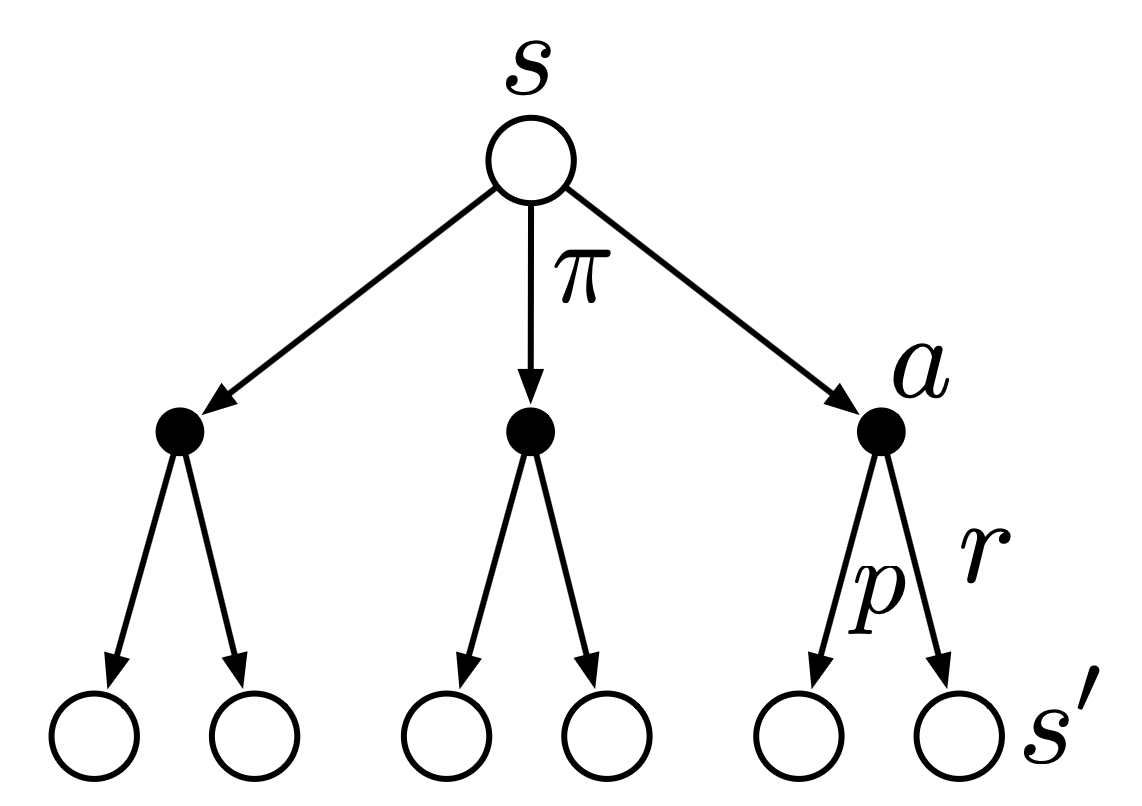
\includegraphics[scale=0.4]{figures/backup_diag.png}
  \caption{DP backup: take the expectation over all immediate successors
    (requires access to the model).}
\end{figure}

\section{Iterative policy evaluation}

Given a fixed policy $\pi$, we want to compute $\vpi$ exactly. The Bellman
expectation equation gives a fixed-point condition: $\vpi = T^{\pi}\vpi$,
where the Bellman expectation \emph{operator} $T^{\pi}$ is:

\begin{defbox}[title={Bellman Expectation Operator}]
\[
  (T^{\pi}v)(s) \;=\; \sum_a \pi(a\mid s)\sum_{s',r} p(s',r\mid s,a)
    \bigl[r + \gamma\,v(s')\bigr].
\]
The true value function $\vpi$ is the unique fixed point satisfying
$T^{\pi}\vpi = \vpi$.
\end{defbox}

Repeated application of $T^{\pi}$ converges to $\vpi$ from any initialization:

\begin{thmbox}[title={Iterative Policy Evaluation (Synchronous)}]
Initialize $V_0$ arbitrarily and iterate:
\[
  V_{k+1}(s) \;=\; (T^{\pi}V_k)(s)
  \;=\; \sum_a \pi(a\mid s)\sum_{s',r} p(s',r\mid s,a)
    \bigl[r + \gamma\,V_k(s')\bigr].
\]
Stop when $\max_s |V_{k+1}(s) - V_k(s)| < \theta$.
\end{thmbox}

\begin{notebox}[title={In-Place (One-Array) Evaluation}]
Update $V(s) \leftarrow (T^{\pi}V)(s)$ immediately, using the most recent
available values for successor states. Convergence is typically \emph{faster}
(Gauss--Seidel style), but the update order can affect intermediate estimates.
Unlike the synchronous version, later states in the same sweep may see
already-updated values from earlier in that sweep.

Iterative policy evaluation is a \textbf{bootstrapping} method: it updates
$V(s)$ using current estimates $V(s')$ of successor states.
\end{notebox}

\section{Policy improvement}

After evaluating $v_\pi$, we can compute the action-value function and look
for a better policy:

\begin{thmbox}[title={Policy Improvement}]
Given $v_\pi$, compute
\[
  q_\pi(s,a) \;=\; \sum_{s',r} p(s',r\mid s,a)\bigl[r + \gamma\,v_\pi(s')\bigr],
\]
and form the greedy policy $\pi'(s) \in \argmax_a\,q_\pi(s,a)$.

\textbf{Policy improvement theorem:} $v_{\pi'}(s) \ge v_\pi(s)$ for all $s$.
The improvement may be strict (genuinely better) or non-strict
($\pi' = \pi$ already, meaning $\pi$ was optimal).
\end{thmbox}

\section{Policy iteration}

Policy iteration alternates between evaluation and improvement until the
policy stabilizes:

\begin{enumerate}
  \item \textbf{Evaluate} the current $\pi$: run iterative evaluation to
    obtain $v_\pi$ (approximately).
  \item \textbf{Improve}: set $\pi \leftarrow \text{Greedy}(q_\pi)$.
  \item Repeat until the policy is unchanged (\emph{policy stable}).
\end{enumerate}

For finite MDPs in the standard discounted setting, policy iteration
terminates at an optimal policy after a finite number of improvements.
\textbf{Modified policy iteration} truncates step 1 to just a few sweeps
before improving, interpolating between policy iteration (full evaluation)
and value iteration (one backup per sweep).

\section{Value iteration}

Instead of evaluating the current policy to convergence, value iteration
applies the \emph{optimality} operator $T^*$ in each sweep:

\begin{thmbox}[title={Value Iteration}]
The Bellman optimality operator:
\[
  (T^*v)(s) \;=\; \max_a \sum_{s',r} p(s',r\mid s,a)\bigl[r + \gamma\,v(s')\bigr].
\]
The fixed point $v_* = T^*v_*$ is the unique optimal value function.

Value iteration iterates $V_{k+1}(s) = (T^*V_k)(s)$ until convergence,
then extracts a greedy optimal policy:
\[
  \pi_*(s) \in \argmax_a \sum_{s',r} p(s',r\mid s,a)\bigl[r + \gamma\,V(s')\bigr].
\]
\end{thmbox}

\begin{intbox}[title={Value Iteration as Policy Iteration with One Backup}]
Value iteration is equivalent to policy iteration where the evaluation step
is truncated to a \emph{single} backup. It implicitly evaluates the greedy
policy w.r.t.\ the current estimate --- without maintaining an explicit policy
variable. Convergence is therefore typically asymptotic, not finite.
\end{intbox}

\section{Asynchronous DP}

Synchronous DP sweeps every state on each pass, which can be expensive.
\textbf{Asynchronous DP} relaxes this: it updates states in any order,
possibly skipping some between passes, applying either the evaluation backup
$V(s) \leftarrow (T^{\pi}V)(s)$ or the optimality backup
$V(s) \leftarrow (T^*V)(s)$. The extreme version is
\textbf{prioritized sweeping}: always update the state with the largest
Bellman residual, so effort is concentrated where estimates are furthest
from being fixed points.

\section{Exam questions}

\begin{exbox}[title={Exam: Optimal Policy via Linear Bellman Equations}]
\textbf{Q.} ``Given an arbitrary policy, the optimal policy can be computed
directly by solving the Bellman equations as a linear system.'' True or false?

\medskip
\textbf{A.} \textbf{False.} The \emph{linear} Bellman system solves $v_\pi$
for a \emph{fixed} $\pi$. Optimality requires a $\max$ (nonlinear condition).
\end{exbox}

\begin{exbox}[title={Exam: Policy Evaluation Computation}]
\textbf{Q.} Policy evaluation with reward $-4$ per step, $\gamma=0.5$, all
initial values $0$, terminal value $0$. What is the value of state 0 after
two sweeps?

\medskip
\textbf{A.} Apply $V_{k+1}(s) = \sum_a \pi(a\mid s)\sum_{s'} p(s'\mid s,a)
[-4 + 0.5\,V_k(s')]$. With $V_0 \equiv 0$: first sweep gives $V_1(s) = -4$
for nonterminal states. Second sweep (example: state 0 transitions to a
nonterminal with prob.\ 0.5 and terminal with prob.\ 0.5):
$V_2(0) = -4 + 0.5\cdot(0.5\cdot(-4) + 0.5\cdot 0) = -5$.
\end{exbox}

\begin{exbox}[title={Exam: Policy Improvement Computation}]
\textbf{Q.} With $R=-1$, $\gamma=1$, compute $Q(\textit{small})$ and
$Q(\textit{large})$ at state 0 and pick the greedy action.

\medskip
\textbf{A.} $Q(a) = \sum_{s'} p(s'\mid 0,a)[-1 + V(s')]$.
\[
  Q(\textit{small}) = 0.5(-1+3)+0.5(-1-1) = 0,
  \quad
  Q(\textit{large}) = 0.5(-1+5)+0.25(-1-3)+0.25(-1-7) = -1.
\]
Greedy choice: \textbf{small}.
\end{exbox}

\begin{notebox}[title={Common Exam Pitfalls — DP}]
\begin{itemize}
  \item Mixing up \textbf{evaluation} (compute $v_\pi$ for fixed $\pi$) with
    \textbf{control} (improve $\pi$ toward optimality).
  \item Forgetting DP is \textbf{model-based}: backups sum over all successors
    using $p(s',r\mid s,a)$.
  \item Confusing \textbf{two-array} (order irrelevant) with \textbf{in-place}
    (order matters) updates.
  \item ``Greedy'' in DP means $\argmax$, not random exploration.
  \item Value iteration: convergence is \textbf{not finite}; use a threshold
    on the Bellman residual to decide when to stop.
\end{itemize}
\end{notebox}


% ==========================================================
\chapter{Monte Carlo Methods}
% ==========================================================

Monte Carlo methods bring model-free learning to the table: they estimate
value functions from \textbf{sampled episodes} of actual (or simulated)
experience, with no knowledge of $p(s',r\mid s,a)$ required. The key
distinction from DP is that MC does \textbf{not bootstrap}: updates are based
on observed returns $G_t$, not on estimates of successor values.

\begin{defbox}[title={Monte Carlo Methods}]
\textbf{MC methods} are model-free and non-bootstrapping: they update value
estimates using complete empirical returns from sampled episodes.
MC typically assumes \textbf{episodic} tasks (or well-defined segments),
because the return
\[
  G_t = \sum_{k=0}^{T-t-1} \gamma^k R_{t+k+1}
\]
requires knowing the trajectory all the way to the terminal step $T$.
\end{defbox}

\section{MC prediction}

Given a fixed policy $\pi$, we estimate $\vpi(s)$ by averaging observed
returns across episodes. The two main variants differ in which visits to count.

\begin{defbox}[title={First-Visit and Every-Visit MC Prediction}]
\textbf{First-visit MC:} for each episode, record the return $G_t$ following
the \emph{first} visit to state $s$, then average across episodes:
$V(s) \leftarrow \text{mean of first-visit returns}$.

\textbf{Every-visit MC:} use the return following \emph{every} visit to $s$
in an episode.

First-visit returns across episodes are i.i.d.\ draws from the same
distribution and converge by the law of large numbers.
Every-visit returns within a single episode are generally \emph{correlated}
(multiple visits share the same trajectory), so they are not i.i.d.,
though every-visit MC still converges asymptotically.
\end{defbox}

The same idea applies to action values: treat each $(s,a)$ pair as the
``state'' and accumulate first-visit (or every-visit) returns for
$Q(s,a) \approx \qpi(s,a)$.

\begin{thmbox}[title={Incremental Mean Update}]
If $V(s)$ is the current mean of $n$ observed returns and a new return $G$
arrives:
\[
  V(s) \leftarrow V(s) + \frac{1}{n+1}\bigl(G - V(s)\bigr).
\]
\end{thmbox}

\begin{exbox}[title={Incremental Update}]
$V(s) = 4$ based on $n=3$ returns; new return $G = 1$:
\[
  V(s) \leftarrow 4 + \tfrac{1}{4}(1-4) = 3.25.
\]
\end{exbox}

\section{MC control}

For control, MC typically estimates \textbf{action values} $Q(s,a)$ rather
than state values, because the greedy improvement step then becomes
$\pi(s) \in \argmax_a Q(s,a)$ --- no model is needed.

\subsection{Exploring starts}

Greedy improvement poses a coverage problem: if the policy never takes action
$a$ in state $s$, $Q(s,a)$ never gets updated, and the policy might get stuck.

\begin{defbox}[title={Exploring Starts (ES)}]
Assume every state--action pair $(s,a)$ can start an episode with nonzero
probability: $\Pr(S_0=s, A_0=a) > 0$ for all $(s,a)$.
This guarantees every pair is eventually tried, so a purely greedy policy
still achieves coverage.
(Primarily a theoretical device; often unrealistic in practice.)
\end{defbox}

\begin{intbox}[title={Why Exploring Starts Are Needed}]
Without ES, a greedy policy that never tries some $(s,a)$ will never correct
$Q(s,a)$. If $Q(s,a)$ is initialized poorly, the policy is stuck.
ES is a clean mathematical hack: by forcing random starts, every pair gets
tried infinitely often in the limit, so $Q$ eventually becomes accurate
everywhere.
\end{intbox}

\subsection{On-policy MC control for $\varepsilon$-soft policies}

A more practical approach uses a policy that always explores a little:

\begin{defbox}[title={$\varepsilon$-Soft Policy}]
$\pi$ is \textbf{$\varepsilon$-soft} if
$\pi(a\mid s) \ge \varepsilon / |\Aset(s)|$ for all $(s,a)$, with $\varepsilon > 0$.
No action is ever completely ruled out, guaranteeing ongoing exploration.
The standard construction is $\varepsilon$-greedy w.r.t.\ $Q$.
\end{defbox}

\begin{intbox}[title={Exploring Starts vs.\ $\varepsilon$-Soft}]
ES injects exploration only at episode \emph{starts}: across many episodes,
every $(s,a)$ is tried as a starting pair.
An $\varepsilon$-soft policy injects exploration \emph{throughout} every
episode: every time state $s$ is visited, every action has nonzero probability.
This prevents ``never tried $\Rightarrow$ never learned'' without requiring
special episode initialization.
\end{intbox}

On-policy MC control repeats: (1) generate an episode under the current
$\varepsilon$-soft policy, (2) update $Q(s,a)$ from observed returns
(first-visit or every-visit), (3) improve $\pi$ to be $\varepsilon$-greedy
w.r.t.\ the updated $Q$. This is generalized policy iteration in the MC
setting.

\section{Off-policy MC and importance sampling}

\begin{defbox}[title={Off-Policy Learning}]
Learn about a \textbf{target policy} $\pi$ using episodes generated by a
different \textbf{behavior policy} $\mu$. Required condition:
\textbf{coverage}: $\mu(a\mid s)=0 \Rightarrow \pi(a\mid s)=0$ for all
$(s,a)$, so that importance sampling ratios are never undefined.
\end{defbox}

\begin{intbox}[title={Why Importance Sampling Is Needed}]
Episodes from $\mu$ contain action choices that $\pi$ would make with
different probabilities. IS reweights each episode so that, in expectation,
it counts as if generated by $\pi$. An episode where $\pi$ is unlikely but
$\mu$ is likely should count \emph{less} (small weight), and vice versa.
\end{intbox}

\begin{thmbox}[title={Importance Sampling Ratio}]
For an episode segment $t$ to $T$:
\[
  \rho_{t:T-1} \;=\; \prod_{k=t}^{T-1}\frac{\pi(A_k\mid S_k)}{\mu(A_k\mid S_k)}.
\]
Then $\rho_{t:T-1}\,G_t$ is an unbiased estimate of $\vpi(S_t)$ under $\mu$.
\end{thmbox}

Because the ratio is a product over many steps, it can become extremely
large or small --- a few rare episodes dominate the average.
\textbf{Ordinary IS} is unbiased but potentially very high variance.
\textbf{Weighted IS} normalizes by total weight, reducing variance at the
cost of a small finite-sample bias:

\begin{thmbox}[title={Ordinary and Weighted Importance Sampling}]
\textbf{Ordinary IS:}
\[
  \hat{v}(s) = \frac{1}{n}\sum_{i=1}^n \rho^{(i)} G^{(i)}.
  \qquad\text{(unbiased, high variance)}
\]
\textbf{Weighted IS:}
\[
  \hat{v}(s) = \frac{\sum_i \rho^{(i)} G^{(i)}}{\sum_i \rho^{(i)}}.
  \qquad\text{(biased for finite $n$, much lower variance)}
\]
Weighted IS is the common practical default.
\end{thmbox}

The weighted IS estimate can be maintained online via cumulative weights
$C(s)$:
\[
  C(s) \leftarrow C(s) + \rho, \qquad
  V(s) \leftarrow V(s) + \frac{\rho}{C(s)}\bigl(G - V(s)\bigr).
\]

\section{Exam questions}

\begin{exbox}[title={Exam: Matching MC Methods}]
\textbf{Q.} Match: (A) $\varepsilon_k=1/k$ for episode $k$;
(B) greedy action with probability $1-\varepsilon$ (constant $\varepsilon$);
(C) learn about $\pi$ from experience generated by $\mu$.
Methods: GLIE MC control; on-policy MC for $\varepsilon$-soft policies;
off-policy learning.

\medskip
\textbf{A.} A $\to$ GLIE MC control;\quad B $\to$ on-policy $\varepsilon$-soft;\quad C $\to$ off-policy.
\end{exbox}

\begin{exbox}[title={Exam: MC Control and State Values}]
\textbf{Q.} ``MC control methods compute an estimate of the state-value
function $v_\pi$.'' True or false?

\medskip
\textbf{A.} \textbf{False (as stated).} MC control is formulated via
\emph{action values} $Q(s,a)$; state values alone are insufficient for
model-free greedy improvement.
\end{exbox}

\begin{exbox}[title={Exam: Coverage Condition}]
\textbf{Q.} In off-policy MC prediction, what condition is needed for
importance sampling to be well-defined?

\medskip
\textbf{A.} \textbf{Coverage:} $\pi(a\mid s) > 0 \Rightarrow \mu(a\mid s)>0$
for all $(s,a)$ that can be visited; otherwise a ratio contains division by zero.
\end{exbox}

\begin{notebox}[title={Common Exam Pitfalls — MC}]
\begin{itemize}
  \item MC is \textbf{model-free} and \textbf{does not bootstrap}; it uses complete returns.
  \item First-visit vs every-visit: every-visit gives more samples per
    episode but within-episode samples are correlated.
  \item For control, MC uses $Q(s,a)$, not just $V(s)$.
  \item Off-policy: the coverage condition is $\mu=0 \Rightarrow \pi=0$
    (not the other way around), and the ratio is a \emph{product} over the
    full trajectory segment.
  \item Ordinary IS is unbiased but numerically unstable;
    weighted IS is the standard practical choice.
\end{itemize}
\end{notebox}


% ==========================================================
\chapter{Temporal Difference Learning}
% ==========================================================

Temporal-difference (TD) learning sits between DP and MC.
Like MC it is \textbf{model-free}, learning from sampled experience.
Like DP it \textbf{bootstraps}: it updates estimates using other learned
estimates rather than waiting for a complete return.
This combination --- online, model-free, bootstrapping --- makes TD the
workhorse of practical RL.

A quick comparison of the three families:
\begin{itemize}
  \item \textbf{DP:} model required; expected backups over all successors.
  \item \textbf{MC:} model-free; no bootstrapping; full episode needed.
  \item \textbf{TD:} model-free; bootstraps from one sampled transition.
\end{itemize}

\section{TD(0) prediction}

\begin{thmbox}[title={TD(0) Target and Error}]
For a transition $S_t \to S_{t+1}$ with reward $R_{t+1}$, the
\textbf{TD(0) target} is $R_{t+1} + \gamma V(S_{t+1})$ and the
\textbf{TD error} is
\[
  \delta_t \;=\; R_{t+1} + \gamma V(S_{t+1}) - V(S_t).
\]
The TD(0) update with step size $\alpha \in (0,1]$:
\[
  V(S_t) \leftarrow V(S_t) + \alpha\,\delta_t.
\]
Only the current state is updated per step (tabular case). If $\gamma=0$,
the target reduces to $R_{t+1}$ (pure immediate reward).
\end{thmbox}

\begin{thmbox}[title={Convergence of Tabular On-Policy TD(0)}]
TD(0) prediction converges to $v_\pi$ if (i) the policy is fixed and
on-policy, (ii) all states are visited infinitely often, and (iii) step sizes
satisfy the Robbins--Monro conditions per state:
\[
  \sum_t \alpha_t(s) = \infty, \qquad \sum_t \alpha_t(s)^2 < \infty.
\]
Off-policy TD and/or function approximation can diverge.
\end{thmbox}

\begin{exbox}[title={TD(0) Update Calculation}]
$V(S_t)=2$, $R_{t+1}=-1$, $\gamma=0.9$, $V(S_{t+1})=3$:
\[
  \delta_t = -1 + 0.9\cdot3 - 2 = -0.3.
\]
With $\alpha=0.1$: $V(S_t) \leftarrow 2 + 0.1(-0.3) = 1.97$.
\end{exbox}

\begin{intbox}[title={Bias--Variance Trade-off}]
TD targets ($R_{t+1} + \gamma V(S_{t+1})$) are typically
\textbf{lower variance} than MC returns --- they use one reward plus a single
estimate rather than a long sum of random rewards. But they are
\textbf{more biased} early on, because $V(S_{t+1})$ is an imperfect
approximation. MC targets are unbiased w.r.t.\ the true return but can have
high variance, especially when episodes are long or rewards are noisy.
\end{intbox}

\begin{notebox}[title={TD vs DP (Exam Nuance)}]
DP uses \emph{expected} backups: it sums over all possible successors using
the model. TD uses \emph{sample} backups: it observes one successor.
In a deterministic environment the sample equals the expectation, so a single
TD step is equivalent to one DP backup. The step size $\alpha$ affects
convergence speed, not the fixed point (for tabular on-policy prediction).
\end{notebox}

\section{TD control}

For control, TD learns \textbf{action values} $Q(s,a)$. The generic TD
control update is:
\[
  Q(S_t,A_t) \leftarrow Q(S_t,A_t)
    + \alpha\Bigl(R_{t+1} + \gamma\,\text{Target}(S_{t+1}) - Q(S_t,A_t)\Bigr).
\]
The target differs between algorithms; that difference defines the key
on-policy/off-policy distinction. For any policy $\pi$:
$v_\pi(s) = \sum_a \pi(a\mid s)\,q_\pi(s,a)$; for deterministic $\pi$,
$v_\pi(s) = q_\pi(s,\pi(s))$.

\subsection{SARSA (on-policy)}

\begin{thmbox}[title={SARSA}]
On-policy TD control: the bootstrap target uses the next action
\emph{actually taken} by the current policy.
\[
  Q(S_t,A_t) \leftarrow Q(S_t,A_t)
    + \alpha\bigl(R_{t+1} + \gamma\,Q(S_{t+1},A_{t+1}) - Q(S_t,A_t)\bigr).
\]
Mnemonic: $(S_t, A_t, R_{t+1}, S_{t+1}, A_{t+1})$.
\end{thmbox}

In practice SARSA runs with an $\varepsilon$-greedy policy to ensure
exploration. Because SARSA is on-policy, the \emph{same} policy both
generates experience and defines the bootstrap target via
$A_{t+1} \sim \pi(\cdot\mid S_{t+1})$.
If $S_{t+1}$ is terminal, set $Q(S_{t+1},\cdot) = 0$.

\subsection{Off-policy SARSA and importance sampling}

\begin{notebox}[title={Off-Policy SARSA}]
To learn about target policy $\pi$ while behaving under $\mu$, apply an IS
correction with ratio $\rho_{t+1} = \pi(A_{t+1}\mid S_{t+1})/\mu(A_{t+1}\mid S_{t+1})$:
\[
  Q(S_t,A_t) \leftarrow Q(S_t,A_t)
    + \alpha\,\rho_{t+1}\bigl(R_{t+1} + \gamma\,Q(S_{t+1},A_{t+1}) - Q(S_t,A_t)\bigr).
\]
Q-learning (below) is off-policy and does \emph{not} require IS, because
its target uses $\max_a Q(S_{t+1},a)$ --- which is policy-agnostic.
\end{notebox}

\subsection{Expected SARSA}

\begin{thmbox}[title={Expected SARSA}]
Replace the sampled $Q(S_{t+1},A_{t+1})$ by its expectation under $\pi$:
\[
  Q(S_t,A_t) \leftarrow Q(S_t,A_t)
    + \alpha\Bigl(R_{t+1} + \gamma\sum_{a}\pi(a\mid S_{t+1})Q(S_{t+1},a)
      - Q(S_t,A_t)\Bigr).
\]
Lower variance than SARSA, since we average over the random next action
instead of sampling it.
\end{thmbox}

\begin{notebox}[title={Expected SARSA vs.\ Q-Learning}]
If the target policy is greedy/deterministic, the expectation collapses to a
max: $\sum_a \pi(a\mid s')Q(s',a) = \max_a Q(s',a)$.
Thus Expected SARSA with a greedy target policy \emph{reduces to Q-learning}.
\end{notebox}

\subsection{Q-learning (off-policy)}

\begin{thmbox}[title={Q-Learning}]
Off-policy TD control: the target uses the \emph{greedy} action at the next
state, independent of the behavior policy:
\[
  Q(S_t,A_t) \leftarrow Q(S_t,A_t)
    + \alpha\bigl(R_{t+1} + \gamma\max_{a}Q(S_{t+1},a) - Q(S_t,A_t)\bigr).
\]
Under standard conditions (all $(s,a)$ updated infinitely often, Robbins--Monro
step sizes), $Q$ converges to $\qstar$ w.p.\ 1.
\end{thmbox}

The \textbf{behavior policy} $\mu$ generates data and should explore (e.g.\
$\varepsilon$-greedy). The \textbf{target policy} $\pi(s)=\argmax_a Q(s,a)$
is the greedy policy being optimized. Although Q-learning is off-policy, no IS
correction is needed: given $(S_t, A_t)$, the next state is sampled from the
environment dynamics, not from $\mu$ or $\pi$. The off-policy nature enters
only through the $\max$ in the backup.

\begin{notebox}[title={Maximization Bias}]
Using $\max_a Q(S_{t+1},a)$ tends to \emph{overestimate} action values in
stochastic settings: the maximum over noisy estimates is systematically
biased upward. \textbf{Double Q-learning} addresses this by maintaining two
estimates $Q_1, Q_2$. For each transition, randomly choose which to update:
the updating network selects the action ($\argmax_a Q_1$), but the other
network evaluates it ($Q_2(s',a^*)$), decorrelating selection from
evaluation.
\end{notebox}

\begin{thmbox}[title={Double Q-Learning}]
On each step, flip a fair coin.
\[
  \text{If heads:} \quad a^* = \argmax_a Q_1(S_{t+1},a), \quad
  Q_1(S_t,A_t) \leftarrow Q_1(S_t,A_t)
    + \alpha\bigl(R_{t+1} + \gamma\,Q_2(S_{t+1},a^*) - Q_1(S_t,A_t)\bigr).
\]
If tails: symmetric with roles of $Q_1$ and $Q_2$ swapped.
The random split decorrelates the two estimates and reduces maximization bias.
\end{thmbox}

\begin{intbox}[title={On-Policy vs.\ Off-Policy in One Line}]
\[
  \text{SARSA:}\quad\text{target uses } A_{t+1} \sim \pi(\cdot\mid S_{t+1})
    \quad\text{(on-policy)}.
\]
\[
  \text{Q-learning:}\quad\text{target uses } \argmax_a Q(S_{t+1},a)
    \quad\text{(off-policy)}.
\]
\end{intbox}

\section{$n$-step TD and the TD--MC spectrum}

$n$-step TD interpolates between TD(0) ($n=1$) and MC ($n=T-t$):

\begin{thmbox}[title={$n$-Step Return}]
\[
  G_t^{(n)} \;=\; R_{t+1} + \gamma R_{t+2} + \cdots
    + \gamma^{n-1}R_{t+n} + \gamma^n V(S_{t+n}).
\]
Then $V(S_t) \leftarrow V(S_t) + \alpha\bigl(G_t^{(n)} - V(S_t)\bigr)$.
Special cases: $n=1$ gives TD(0); $n = T-t$ removes the bootstrap term and
recovers MC.
\end{thmbox}

$n$-step TD can update before episode end: once $n$ rewards have been
observed, the partial trajectory suffices.
If $n$ exceeds the remaining episode length, the target becomes the full
return (MC), not DP.

\section{Eligibility traces and TD($\lambda$)}

Rather than committing to a single $n$, TD($\lambda$) mixes all $n$-step
returns with geometrically decaying weights.

\begin{thmbox}[title={$\lambda$-Return (Forward View)}]
\[
  G_t^{\lambda} = (1-\lambda)\sum_{n=1}^{T-t-1}\lambda^{n-1} G_t^{(n)}
    + \lambda^{T-t-1} G_t.
\]
Special cases: $\lambda=0$ gives TD(0); $\lambda \to 1$ approaches MC.
\end{thmbox}

The forward view requires knowing the full future, making it online-unfriendly.
Eligibility traces provide an equivalent \emph{backward view}:

\begin{thmbox}[title={Eligibility Traces (Backward View)}]
For state values, maintain traces $e_t(s)$:
\[
  e_t(s) = \gamma\lambda\,e_{t-1}(s) + \mathbf{1}\{S_t=s\}.
\]
Update all states proportionally to their trace:
\[
  V(s) \leftarrow V(s) + \alpha\,\delta_t\,e_t(s)\quad\text{for all }s.
\]
For action values: $e_t(s,a) = \gamma\lambda\,e_{t-1}(s,a) + \mathbf{1}\{S_t=s,A_t=a\}$,
with $Q(s,a) \leftarrow Q(s,a) + \alpha\,\delta_t\,e_t(s,a)$. The TD error
$\delta_t$ depends on whether the underlying algorithm is SARSA,
Expected SARSA, or Q-learning.
\end{thmbox}

\begin{notebox}[title={Batch TD vs.\ Batch MC}]
In the tabular case, batch TD(0) converges to the value function of the
\textbf{maximum-likelihood Markov model} implied by the data (the DP solution
on empirical transition dynamics). Batch MC converges to the solution
minimizing mean-squared error on the observed returns. They generally converge
to \emph{different} solutions.

With \textbf{function approximation and bootstrapping} (semi-gradient TD,
TD($\lambda$), etc.), convergence is \emph{not} guaranteed in general.
\end{notebox}

\section{Exam questions}

\begin{exbox}[title={Exam: TD vs.\ MC}]
\textbf{Q.} What is an advantage of TD learning over Monte Carlo methods?

\medskip
\textbf{A.} TD updates \textbf{online} after each step --- no need to wait for
episode end. This often yields faster learning in practice and works for
continuing (non-episodic) tasks.
\end{exbox}

\begin{exbox}[title={Exam: SARSA On-Policy}]
\textbf{Q.} ``SARSA requires choosing a second action in the second state with
the same policy as the first.'' True or false?

\medskip
\textbf{A.} \textbf{True.} SARSA is on-policy: it needs
$A_{t+1} \sim \pi(\cdot\mid S_{t+1})$ to form the target $Q(S_{t+1},A_{t+1})$.
\end{exbox}

\begin{exbox}[title={Exam: TD($\lambda$)}]
\textbf{Q.} ``TD($\lambda$) computes a weighted average $n$-step TD backup
target.'' True or false?

\medskip
\textbf{A.} \textbf{True.} The $\lambda$-return is a geometric mixture of
$n$-step returns (forward view), implemented efficiently via eligibility
traces (backward view).
\end{exbox}

\begin{notebox}[title={Common Exam Pitfalls — TD}]
\begin{itemize}
  \item \textbf{Bootstrapping:} TD uses $V(S_{t+1})$ or $Q(S_{t+1},\cdot)$
    inside the target; MC does not.
  \item \textbf{SARSA vs.\ Q-learning:} SARSA uses the \emph{actually taken}
    $A_{t+1}$ (on-policy); Q-learning uses $\max_a$ (off-policy).
  \item Expected SARSA takes an expectation \emph{under the policy} at
    $S_{t+1}$; with a greedy target policy it reduces to Q-learning.
  \item Endpoints: $\lambda=0 \Rightarrow$ TD(0); $\lambda \to 1 \Rightarrow$ MC.
  \item Eligibility traces \textbf{decay} by $\gamma\lambda$ and assign
    credit backward to recently visited states / state--action pairs.
\end{itemize}
\end{notebox}


% ==========================================================
\chapter{Policy Gradient Methods}
% ==========================================================

Value-based methods (Q-learning, SARSA) represent the policy implicitly
via a value function: act greedily. \textbf{Policy gradient methods}
instead parameterize the policy directly and optimize it by gradient ascent
on an objective $J(\theta)$. This is natural for continuous action spaces
(where $\argmax_a Q(s,a)$ is hard), for stochastic policies, and wherever
a differentiable policy representation is available.

\section{The policy gradient objective}

\begin{defbox}[title={Parameterized Policy and Objective}]
A \textbf{policy gradient (PG) method} optimizes $\pi_\theta(a\mid s)$
directly by gradient ascent:
$\theta \leftarrow \theta + \alpha\,\nabla_\theta J(\theta)$.
A common objective is the expected discounted return from a start-state
distribution:
\[
  J(\theta) = \E_{\tau \sim \pi_\theta}\!\left[\sum_{t=0}^{T-1}\gamma^t R_{t+1}\right],
\]
where $\tau = (S_0, A_0, R_1, S_1, \dots)$ is a trajectory induced by $\pi_\theta$.
\end{defbox}

\section{REINFORCE}

The key mathematical tool is the \emph{log-derivative trick}:

\begin{thmbox}[title={Score Function / Log-Derivative Identity}]
\[
  \nabla_\theta\,\pi_\theta(a\mid s)
  = \pi_\theta(a\mid s)\,\nabla_\theta\log\pi_\theta(a\mid s).
\]
Applying this inside the expectation over trajectories yields the policy
gradient theorem:
\[
  \nabla_\theta J(\theta)
  \propto \E_{\pi_\theta}\!\left[\sum_t
    \nabla_\theta\log\pi_\theta(A_t\mid S_t)\,q_{\pi_\theta}(S_t,A_t)\right].
\]
No knowledge of the environment dynamics $p(s',r\mid s,a)$ is needed.
\end{thmbox}

Replacing $q_{\pi_\theta}$ with the observed Monte Carlo return $G_t$ gives
the REINFORCE algorithm:

\begin{thmbox}[title={REINFORCE (MC Policy Gradient)}]
After completing an episode, for each time step $t$:
\[
  \theta \leftarrow \theta + \alpha\,G_t\,\nabla_\theta\log\pi_\theta(A_t\mid S_t).
\]
Increase the probability of actions that led to high return; decrease it for
actions with low return.
\end{thmbox}

REINFORCE is an \textbf{unbiased} estimator of $\nabla_\theta J(\theta)$ but
can have \textbf{high variance}, especially in long episodes. It is also
\textbf{on-policy}: trajectories must come from the current $\pi_\theta$.

\begin{notebox}[title={Course/Exam Convention}]
In this course, REINFORCE refers to the \textbf{episodic Monte Carlo} variant
that uses full episode returns $G_t$. The claim ``REINFORCE is effective for
both episodic and non-episodic MDPs'' is therefore \textbf{false} under this
convention: continuing tasks require additional machinery (average-reward
formulations or actor--critic with TD critics).
\end{notebox}

\section{Baselines and variance reduction}

\begin{thmbox}[title={Baseline Trick}]
For any function $b(s)$ that does not depend on the action $A_t$:
\[
  \E_{\pi_\theta}\!\left[b(S_t)\,\nabla_\theta\log\pi_\theta(A_t\mid S_t)\right] = 0.
\]
Therefore $G_t$ can be replaced by $G_t - b(S_t)$ without changing the
expected gradient, but typically reducing variance (the baseline shifts all
action probabilities equally in expectation, canceling out):
\[
  \theta \leftarrow \theta
    + \alpha\,(G_t - b(S_t))\,\nabla_\theta\log\pi_\theta(A_t\mid S_t).
\]
Common baselines: $b(s) = \bar{G}$ (running mean return), or
$b(s) = V_w(s)$ (a learned state-value function).
\end{thmbox}

\begin{defbox}[title={Advantage Function}]
When $b(s) = v_\pi(s)$, the quantity $G_t - b(S_t)$ estimates the
\textbf{advantage}:
\[
  A_\pi(s,a) = q_\pi(s,a) - v_\pi(s).
\]
The advantage answers ``how much better than average was action $a$ in state
$s$?'' --- a cleaner and lower-variance learning signal.
\end{defbox}

If $b(s) = V_w(s)$ is itself learned, the setup is called
\textbf{actor + critic}. It is \emph{not} a TD method unless the critic is
trained with TD targets (e.g.\ using $\delta_t$).

\section{Actor--critic}

\textbf{Actor--critic} methods combine an \textbf{actor}
(the parameterized policy $\pi_\theta$) with a \textbf{critic} (a value
estimator $V_w$ or $Q_w$). The critic provides a TD-style learning signal to
update the actor; the actor update only needs the scalar $\delta_t$ or
$\hat{A}_t$ from the critic --- it does not need $\nabla_w V_w$.

The one-step TD error serves as an advantage estimate:

\begin{thmbox}[title={Actor--Critic Updates}]
\textbf{Critic} (TD(0) on $V_w$):
\[
  \delta_t = R_{t+1} + \gamma\,V_w(S_{t+1}) - V_w(S_t), \qquad
  w \leftarrow w + \beta\,\delta_t\,\nabla_w V_w(S_t).
\]
\textbf{Actor:}
\[
  \theta \leftarrow \theta + \alpha\,\delta_t\,\nabla_\theta\log\pi_\theta(A_t\mid S_t).
\]
\end{thmbox}

\begin{intbox}[title={REINFORCE vs.\ Actor--Critic}]
Compared to REINFORCE, actor--critic can update \textbf{online} (no waiting
for episode end) and typically has lower variance. The cost is
\textbf{bias} introduced by bootstrapping from the approximate critic.
This is the classic bias--variance trade-off that runs through all of RL.
\end{intbox}

\subsection{PPO (brief)}

\begin{thmbox}[title={Proximal Policy Optimization (PPO)}]
PPO stabilizes policy updates via a \textbf{clipped surrogate} objective.
With probability ratio $r_t(\theta) = \pi_\theta(A_t\mid S_t) /
\pi_{\theta_\text{old}}(A_t\mid S_t)$:
\[
  L^\text{CLIP}(\theta) = \E\!\left[\min\bigl(r_t(\theta)\hat{A}_t,\;
    \mathrm{clip}(r_t(\theta),\,1-\epsilon,\,1+\epsilon)\hat{A}_t\bigr)\right].
\]
Clipping prevents any single update from moving the policy too far from
$\pi_{\theta_\text{old}}$, stabilizing training without a hard constraint.
\end{thmbox}

\section{Exam questions}

\begin{exbox}[title={Exam: Baseline Unbiasedness}]
\textbf{Q.} Why can we subtract a baseline $b(S_t)$ from the return in
REINFORCE without biasing the gradient?

\medskip
\textbf{A.} Because $\E[b(S_t)\nabla_\theta\log\pi_\theta(A_t\mid S_t)] = 0$
under $A_t \sim \pi_\theta(\cdot\mid S_t)$, so the baseline term vanishes in
expectation and does not affect $\E[\nabla_\theta J(\theta)]$.
\end{exbox}

\begin{exbox}[title={Exam: REINFORCE Variance}]
\textbf{Q.} ``REINFORCE is unbiased but often high variance.'' True or false?

\medskip
\textbf{A.} \textbf{True.} It uses Monte Carlo returns; variance can be large
without baselines or critics.
\end{exbox}

\begin{exbox}[title={Exam: Online Actor--Critic}]
\textbf{Q.} ``Actor--critic methods can update before an episode ends.''
True or false?

\medskip
\textbf{A.} \textbf{True.} The critic provides a TD-style signal that
bootstraps from the next state, enabling online updates after every step.
\end{exbox}

\begin{notebox}[title={Common Exam Pitfalls — Policy Gradients}]
\begin{itemize}
  \item PG is \textbf{gradient ascent} on $J(\theta)$, not descent.
  \item Updates use $\nabla_\theta\log\pi_\theta(A_t\mid S_t)$, not
    $\nabla_\theta\pi_\theta$ directly.
  \item The baseline must not depend on the chosen action; otherwise it
    introduces bias.
  \item Actor--critic reduces variance but introduces bias (bootstrapping);
    REINFORCE is unbiased but high variance.
  \item $G_t$ is the MC return; $\delta_t$ is the TD error / one-step
    advantage estimate --- do not confuse them.
  \item With expert state--action pairs $(s,a)$, a policy can be pre-trained
    via supervised learning ($\max_\theta \log\pi_\theta(a\mid s)$) before
    RL fine-tuning.
\end{itemize}
\end{notebox}


\backmatter
\end{document}
